\section{Sharpness}\label{sec:sharpness}

Let \(\theta^{\ast}\in\reals^{d}\) be a local minimum of \(f\).
The sharpness of the loss landscape at \(\theta^{\ast}\)
quantifies how quickly the loss increases away from \(\theta^{\ast}\).
Intuitive, empirical, and theoretical observations suggest that
sharpness and generalization are linked,
more specifically, sharpness is negatively correlated with generalization
(see \Cref{fig:sharpvflat},~\citealt{keskarLargeBatchTrainingDeep2022}).
\begin{figure}[htb]
	\begin{center}
		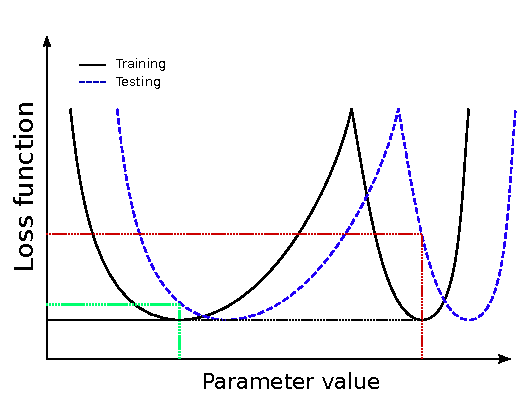
\includegraphics[width=0.6\linewidth]{pdf/sharpvflat.pdf}
	\end{center}
	\caption{%
		The flat minimum (left) performs similarly on both training and test data,
		while the sharp minimum (right) performs poorly on test data: it overfits%
		~\cite{keskarLargeBatchTrainingDeep2022}.
	}\label{fig:sharpvflat}
\end{figure}

\subsection{Notions of sharpness}\label{sub:sharpness:notions}

Sharpness, and its converse, flatness,
have been of interest to \gls{abb:ml} researchers for at least since the late 1990s%
~\cite{hochreiterFlatMinima1997}.
Consequently, the community has had time to introduce a panoply
of distinct, yet related notions of sharpness.
In this section we present a non-exhaustive list of such notions,
the interactions therebetween, and the relationship to generalization.

The earliest attempts at quantifying sharpness are based on zeroth-order information
on the function's variation in a neighborhood around a local minimum.
In this vein, \citet{hochreiterFlatMinima1997} introduce
the \(\epsilon\)-flatness (\(\epsilon \gt 0\)) at a local minimum \(\theta^{\ast}\) as
the volume of the largest (for inclusion) connected set \(A \subset \reals^{d}\) such that
\(\theta^{\ast}\in A \) and
\begin{equation}\label{eq:sharpness:epsflatness}
	\forall \theta\in A, \quad f(\theta) \leq f(\theta^{\ast}) + \epsilon.
\end{equation}
Larger volume for smaller \(\epsilon\) indicates a flatter minimum.
\citet{keskarLargeBatchTrainingDeep2022} take the dual perspective,
constraining the volume and using the loss to measure sharpness.
This yields the following definition of what they call \(\epsilon\)-sharpness
\begin{equation}\label{eq:sharpness:epsharpness}
	\max_{\lpnorm[\infty]{\theta - \theta^{\ast}}\le\epsilon}%
	{\frac{f(\theta) - f\left( \theta^{\ast} \right)}{1+f(\theta^{\ast})}}.
\end{equation}
Both of these definitions share a glaring weakness: they cannot handle bounded functions
(see \Cref{fig:epsflat_counterexample}).
\begin{figure}[hbt]
	\begin{center}
		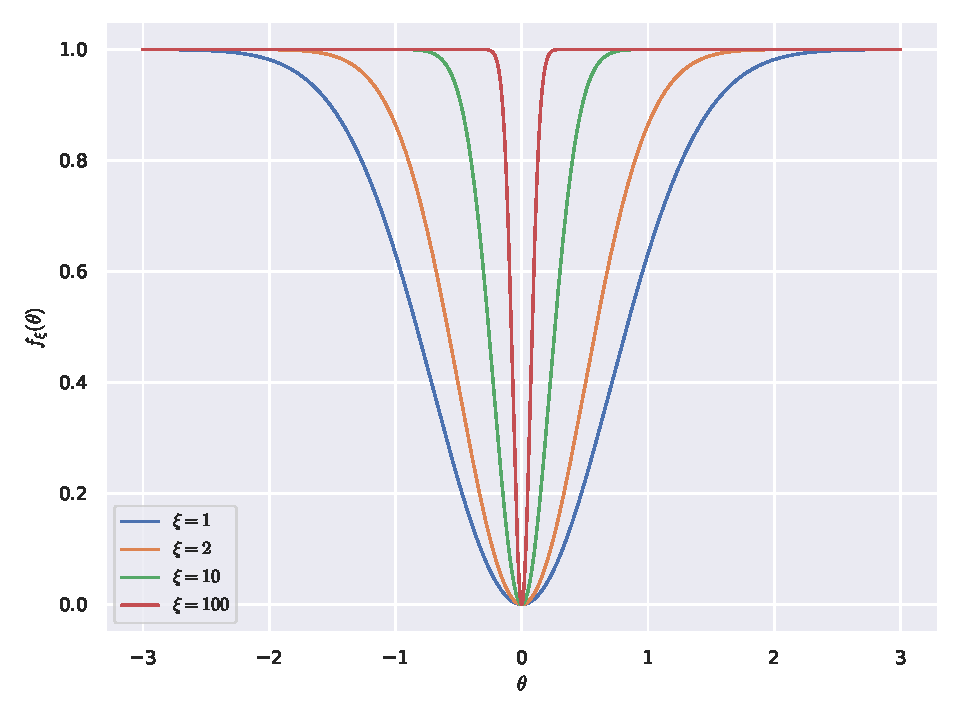
\includegraphics[width=0.6\linewidth]{python/pdf/epsflat_counterexample.pdf}
	\end{center}
	\caption{%
		All functions \(f_{\xi}\) are infinitely \(1\)-flat, and \(1\)-sharp at \(\theta^{\ast} = 0\)
		despite looking visually sharper for larger \(\xi\).
	}\label{fig:epsflat_counterexample}
\end{figure}

Other authors resorted to the use of second-order curvature to define sharpness.
Most notably, functions of the spectrum of the loss Hessian matrix
like the trace~\cite{%
	yangTaxonomizingLocalGlobal2021,%
	petzkaRelativeFlatnessGeneralization2021,%
	ibayashiMinimumSharpnessScaleinvariant2021,%
	leeNewCharacterizationEdge2022,%
	petzkaReparameterizationInvariantFlatnessMeasure2019%
}, the spectral norm%
~\cite{yangTaxonomizingLocalGlobal2021,kaurMaximumHessianEigenvalue2023},
and, more generally, the eigenvalue distribution~\cite{%
	keskarLargeBatchTrainingDeep2022,%
	chaudhariEntropySGDBiasingGradient2019%
}.
These measures are not a complete departure from the zeroth-order sharpness measures,
as, for example, \(\epsilon\)-sharpness is approximated by the formula
\[
	\frac{\lambda_{1}\epsilon^{2}}{2 \left( 1+f\left( \theta^{\ast} \right) \right)},
\]
for small \(\epsilon\), where \(\lambda_{1}\) is the maximum eigenvalue of the Hessian
(i.e.,\ the spectral norm)%
~\cite{keskarLargeBatchTrainingDeep2022,zhangWhyFlatnessDoes2021,dinhSharpMinimaCan2017}.
All the metrics introduced so far%
~\cite[including the zeroth-order ones][]{ibayashiMinimumSharpnessScaleinvariant2021}
suffer from a common problem: they are parameter dependent%
~\cite{%
	dinhSharpMinimaCan2017,%
	jangReparametrizationInvariantSharpnessMeasure2022,zhangWhyFlatnessDoes2021,%
	liangFisherRaoMetricGeometry2019%
}.
Sharpness however, is a geometric property, and must be invariant to re-parametrization.

To address this, multiple metrics have been introduced
with invariance to certain classes of transformations.
Relative flatness~\cite{petzkaRelativeFlatnessGeneralization2021}
is one such metric, defined using both parameters and the Hessian,
which is invariant to neuron-wise (and by extension layer-wise) scaling.
Minimum sharpness~\cite{ibayashiMinimumSharpnessScaleinvariant2021}
is similarly invariant to layer-wise scaling.
Defined as the smallest trace of the Hessian over all layer-wise rescalings
that leave the model unchanged, it achieves scale invariance more or less by definition.
The Fisher-Rao norm~\cite{liangFisherRaoMetricGeometry2019},
defined as
\(
\lpnorm[I(\theta^{\ast})]{\theta^{\ast}}^{2} =
\transpose{{\theta^{\ast}}}I(\theta^{\ast})\theta^{\ast}
\),
where \(I(\theta^{\ast})\) is the Fisher information matrix,
is motivated by information geometry and is in fact \emph{intrinsic},
i.e.,\ identical for different parametrizations of the same model.
Pushing this idea further, \citet{jangReparametrizationInvariantSharpnessMeasure2022}
propose another information-geometric sharpness measure,
which is invariant to arbitrary smooth reparametrizations.
Finally, \citet{zhangWhyFlatnessDoes2021} bypass the issue of parameterization altogether,
by directly defining sharpness in function space.
More concretely, the sharpness of a model is the prior probability that
\gls{abb:sgd} will converge to it from a random initialization.

\subsection{Sharpness and generalization}\label{sub:sharpness:generalization}

According to \citet{keskarLargeBatchTrainingDeep2022,hochreiterFlatMinima1997},
sharpness (as defined in \Cref{eq:sharpness:epsflatness,eq:sharpness:epsharpness})
is negatively correlated with generalization.
Empirical results and theoretical arguments are advanced to support this claim.
\citet{sunExploringVulnerabilityDeep2021} further argue that sharpness is connected
to vulnerability to adversarial attacks.
However, this view is challenged by \citet{dinhSharpMinimaCan2017},
who demonstrate that these measures are scale dependent,
even when the scaling leaves the model unchanged.
For \(\relu\)-activated networks, homogeneity means that this dependence implies
any parameter vector is equivalent to an arbitrarily sharp one, making these measures meaningless.

Some authors attempt to address this by making their sharpness measures invariant to scaling
and other transformations~\cite{%
	ibayashiMinimumSharpnessScaleinvariant2021,%
	petzkaRelativeFlatnessGeneralization2021,%
	liangFisherRaoMetricGeometry2019,%
	jangReparametrizationInvariantSharpnessMeasure2022%
}.
Some of them directly incorporate the group of transformations in the definition of sharpness%
~\cite{%
	ibayashiMinimumSharpnessScaleinvariant2021,%
	kwonASAMAdaptiveSharpnessAware2021%
},
while others appeal to concepts from differential geometry and information geometry%
~\cite{%
	liangFisherRaoMetricGeometry2019,%
	jangReparametrizationInvariantSharpnessMeasure2022%
}.

Other authors~\cite{zhangWhyFlatnessDoes2021,andriushchenkoModernLookRelationship2023}
build on the observations in~\citet{dinhSharpMinimaCan2017},
to argue that sharpness is not the right measure to look at.
\citet{andriushchenkoModernLookRelationship2023} in particular,
find appealing evidence that the correct measure of sharpness is highly dependent on the data.

\subsection{Addressing sharpness}\label{sub:sharpness:addressing}

The connection between sharpness and generalization motivated the development of
multiple algorithms that aim to improve generalization by minimizing sharpness.
Most prominent among these, is \gls{abb:sam}~\cite{foretSharpnessawareMinimizationEfficiently2020},
which adds a sharpness term similar to \(\epsilon\)-sharpness to the loss function.
Experiments on multiple benchmarks show generalization improvements,
and an explicit generalization bound involving the sharpness term is proven.
A number of follow-up works have been published, building on the success of \gls{abb:sam}
by adding invariance to the sharpness measure~\cite{%
	kwonASAMAdaptiveSharpnessAware2021,%
	ibayashiMinimumSharpnessScaleinvariant2021%
},
providing insights into its mechanism~\cite{%
	tahmasebiUniversalClassSharpnessAware2024,%
	andriushchenkoUnderstandingSharpnessAwareMinimization2022%
},
and extending it to \gls{abb:fl}~\cite{caldarolaImprovingGeneralizationFederated2022}.

Despite \gls{abb:sam}'s success, it is not the only algorithm that aims to minimize sharpness.
Entropy-SGD~\cite{chaudhariEntropySGDBiasingGradient2019} is another such algorithm.
Instead of adding a sharpness term to the loss function,
it produces a smoothed version that is less sharp.
This alternate objective is minimized using Langevin dynamics,
which leads to a nested optimization problem.

